\section{Durchführung}
\label{sec:Durchführung}


\subsection{Versuchsaufbau}

Zur Aufnahme der Kennlinien wird der nach \autoref{fig:abb7} aufgebaute Versuchsaufbau verwendet. 
Lediglich der XY-Schreiber wird aus dem Aufbau entfernt.

\begin{figure}[H]
    \centering
    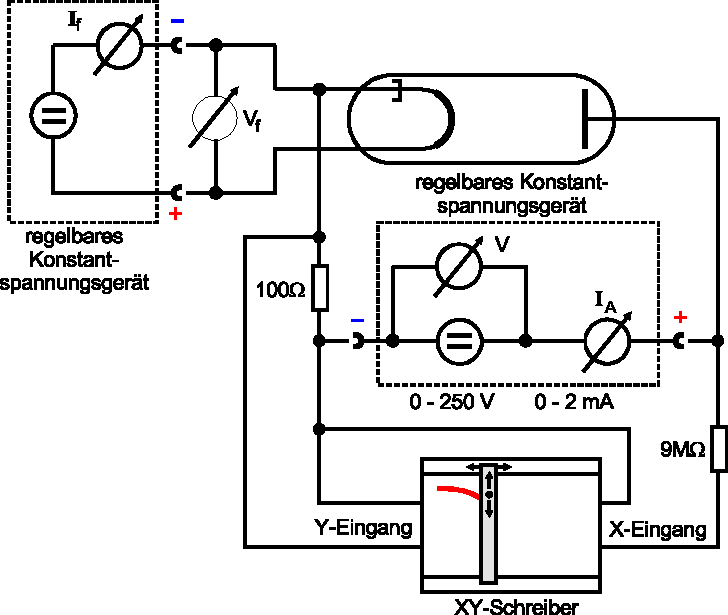
\includegraphics[width = 0.75\textwidth]{figures/Abb7.pdf}
    \caption{Schematischer Versuchsaufbau zur Bestimmung der Kennlinien \cite{ap09}.}
    \label{fig:abb7}
\end{figure}

Die Heizspannung $U_\text{f}$ und der Heizstrom $I_\text{f}$ werden dabei einem Volt- bzw. Amperemeter abgelesen werden.
Die Anodenspannung $U$, die aus dem Konstantspannungsgerät gespeist wird, sowie der Anodenstrom $I_\text{A}$ lassen sich an einem weiteren Volt- und Amperemeterpaar ablesen. \\

Um den Anlaufstrom zu messen, wird der Versuchsaufbau \autoref{fig:abb8} umgebaut.

\begin{figure}[H]
    \centering
    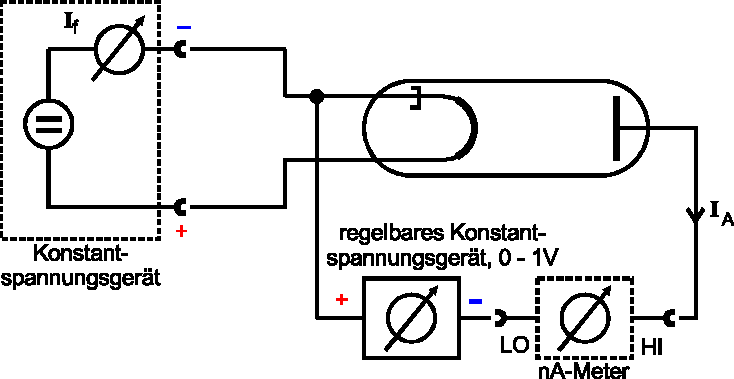
\includegraphics{figures/Abb8.pdf}
    \caption{Schematischer Versuchsaufbau zur Bestimmung des Anlaufstroms \citeyear{ap09}.}
    \label{fig:abb8}
\end{figure}


\subsection{Versuchsdurchführung}

Zunächst wird ein Wertepaar aus Anodenstrom und Anodenspannung aufgenommen.
Es ist wichtig, darauf zu achten, dass die die Toleranzgrenze der hier verwendeten Apparatur bei $2,5 \,\unit{\ampere}$ liegt, der Strom also im jedem Fall kleiner sein muss.
Nun wird die Heizspannung erhöht, bis sich ein Sättigungsprozess zeigt.
Die Heizspannung mit dem dazugehörigen Heizstrom werden als weiteres Wertepaar aufgenommen.
Danach wird die Messung für vier weitere Anodenstrom und -spannungspaare wiederholt. \\

Zur Aufnahme des Anlaufstroms wird die vorher verwendete Spannungsquelle umgepolt und anschließend in $0,05 \,\unit{\volt}$-Schritten erhöht, sodass zu jeder Spannung der Strom abgelesen werden kann.
